%\documentclass[PhD,two side]{srmuthesis}
%\documentclass[MS]{srmuthesis}
%\documentclass[MTech]{srmuthesis}
\documentclass[BTech]{srmuthesis}
\usepackage{array}
\usepackage{times}
\usepackage{t1enc}
\usepackage{tikz}
\usepackage{subfigure}
\usepackage{pgfplots}
\usepackage{setspace} 
\usepackage{enumitem}
\usepackage{geometry}
\usepackage{graphicx}
\usepackage{epstopdf}
\usepackage{lscape}
\usepackage{listings}
\usepackage{fancyhdr}
\usepackage{float}
\usepackage{natbib}
\usepackage[hidelinks=true]{hyperref} % hyperlinks for references.
\usepackage{amsmath} % easier math formulae, align, subequations \ldots
\usepackage{amssymb}
\usepackage{wasysym}
\usepackage{titlesec}
\usepackage{tabularx}
\usepackage{textcomp}
\usepackage{pifont}
\usepackage{appendix} 
\usetikzlibrary{decorations.pathmorphing}
\usetikzlibrary{shapes,arrows,shadows,patterns}
\usepackage[printonlyused]{acronym}
%\usepackage{nomencl}
%\newcommand{\bigsize}{\fontsize{16pt}{20pt}\selectfont}
%\renewcommand\nomname{\centerline {NOTATION}}
%\makenomenclature
\setcounter{MaxMatrixCols}{20}
\captionsetup[figure]{labelfont=bf}
\begin{document}
%%%%%%%%%%%%%%%%%%%%%%%%%%%%%%%%%%%%%%%%%%%%%%%%%%%%%%%%%%%%%%%%%%%%%%
%Cite all
\nocite{thirteen, fifteen, sixteen, seventeen, eighteen, tim, rf, keras, tf, lstm, momoh, lstm1, genetic1, forest123}
%%%%%%%%%%%%%%%%%%%%%%%%%%%%%%%%%%%%%%%%%%%%%%%%%%%%%%%%%%%%%%%%%%%%%%
% Title page

\title{Forecasting Share Prices Using Soft Computing Techniques} % Enter The Project Title

\firstauthor{ G. Vignesh }% Enter The Student name
\firstauthorregno{[Reg No:RA1511003010323]}
\secondauthor{}% Enter The Student name
\secondauthorregno{}
\thirdauthor{} % If there is no third author, leave the space blank like \thirdauthor{}
\thirdauthorregno{}
\fourthauthor{}
\fourthauthorregno{}
\fifthauthor{}
\fifthauthorregno{}
\guide{Mrs. Aswathy K. Cherian} % Enter your guide's name
\designation{Assistant Professor} % Enter your guide's designation
\guidedepartment{Computer Science and Engineering} % Enter the department name of your Guide 
\hod{Dr. B. Amutha} % Enter HOD's name
\department{Computer Science and Engineering} % Enter your department name
\date{MAY 2019} % Enter month and year of submission
%\nocite{*}

\maketitle
%%%%%%%%%%%%%%%%%%%%%%%%%%%%%%%%%%%%%%%%%%%%%%%%%%%%%%%%%%%%%%%%%%%%%%
%\vspace*{3in}
%\begin{center}
%{\Huge Dedicated to my Parents}
%\end{center}
%%%%%%%%%%%%%%%%%%%%%%%%%%%%%%%%%%%%%%%%%%%%%%%%%%%%%%%%%%%%%%%%%%%%%%
% Certificate
\certificate

%\vspace*{0.5in}



%%%%%%%%%%%%%%%%%%%%%%%%%%%%%%%%%%%%%%%%%%%%%%%%%%%%%%%%%%%%%%%%%%%%%%
% Abstract
\abstract
\begin{doublespacing}
\noindent For a long time, there has been the trend of trading of stocks. Brokerage firms and dealers buy/sell stocks for clients and companies. Their work is based on knowing how the share price of the company will react in the market. Market/share price predictions are useful as the investor/broker can attempt to predict the output in order to maximize his dividends or minimize his losses. Prediction of financial market has become easier in this digital age. With the help of high performance computing, we can now work faster and on a larger scale. Prediction of financial markets is especially useful for trader/brokers/investors, who would like to increase their profits by deciding the appropriate action based on market behavior. Using data mining techniques, an attempt is made to estimate a prediction model to help forecast stock prices. R and Python will be the tools used to sort, segregate and process the data, and techniques/algorithms such as \ac{GA}, \ac{ARIMA}, Holt Winters, Linear Regression, \ac{ANN} etc. will be used to forecast results of data. The data has been taken from website of NSE INDIA. Along with the model data, external factors affecting stock prices will also be taken into account. The result will be compared with actual prices and the difference in error will be recorded. R, Python and Weka will be used to create, test and evaluate the models.
\end{doublespacing}
\pagebreak
%%%%%%%%%%%%%%%%%%%%%%%%%%%%%%%%%%%%%%%%%%%%%%%%%%%%%%%%%%%%%%%%%%%%%%
% Acknowledgements
\acknowledgements
I express my humble gratitude to {\bf Dr. Sandeep Sancheti}, Vice Chancellor, SRM Institute of Science and Technology, for the facilities extended for the project work and his continued support.\\ \\
I extend my sincere thanks to {\bf Dr. C. Muthamizhchelvan}, Director, Faculty of Engineering and Technology, SRM Institute of Science and Technology, for his invaluable support.

I wish to thank {\bf Dr. B. Amutha}, Professor \& Head, Department of Computer Science and Engineering, SRM Institute of Science and Technology, for her valuable suggestions and encouragement throughout the period of the project work.

I am extremely grateful to my Academic Advisor {\bf Dr. K. Annapurani}, Associate Professor, Department of Computer Science and Engineering, SRM Institute of Science and Technology, for her great support at all the stages of project work.

I would like to convey my thanks to our Panel Head, {\bf Dr. E. Poovammal}, Professor, Department of Computer Science and Engineering, SRM Institute of Science and Technology, for her inputs during the project reviews.

I register my immeasurable thanks to my Faculty Advisor, {\bf Mrs. P. Mahalakshmi}, Assistant Professor, Department of Computer Science and Engineering, SRM Institute of Science and Technology, for leading and helping my to complete my course.

My inexpressible respect and thanks to my guide, {\bf Mrs. Aswathy K. Cherian}, Assistant Professor, Department of Computer Science and Engineering, SRM Institute of Science and Technology, for providing me an opportunity to pursue my project under her mentorship. She provided me the freedom and support to explore the research topics of my interest. Her passion for solving the real problems and making a difference in the world has always been inspiring.

I sincerely thank staff and students of the Computer Science and Engineering Department, SRM Institute of Science and Technology, for their help during my research. Finally, I would like to thank my parents, my family members and my friends for their unconditional love, constant support and encouragement.

\begin{flushright}
	{\bf G. Vignesh}
\end{flushright}
%%%%%%%%%%%%%%%%%%%%%%%%%%%%%%%%%%%%%%%%%%%%%%%%%%%%%%%%%%%%%%%%%
% Table of contents etc.

\begin{singlespace}
	\tableofcontents
	\thispagestyle{empty}
	
	\listoftables
	\addcontentsline{toc}{chapter}{LIST OF TABLES}
	\listoffigures
	\addcontentsline{toc}{chapter}{LIST OF FIGURES}
\end{singlespace}


%%%%%%%%%%%%%%%%%%%%%%%%%%%%%%%%%%%%%%%%%%%%%%%%%%%%%%%%%%%%%%%%%%%%%%
\abbreviations
%\begin{acronym}[longest acronym must be entered here]
\begin{acronym}[OKID/ERA]
	
	%\acro{acronym}{in detail}
	\acro{ANN}{Artificial Neural Networks}
	\acro{GA}{Genetic Algorithm}
	\acro{KLD}{Kullback Leibler Divergence}
	\acro{ARIMA}{Auto Regressive Integrated Moving Average}
	\acro{LSTM}{Long Short Term Memory}
	\acro{SVM}{Support Vector Machine}
	\acro{RNN}{Recurrent Neural Netowrk}
	\acro{NSE}{National Stock Exchange}
	\acro{NIFTY50}{National Stock Exchange Fifty}
	\acro{BSE}{Bombay Stock Exchange}
	\acro{RF}{Random Forest}
\end{acronym}
% Use the syntax \ac{acronym} whereever you use this acronym.
% Abbreviations

%\noindent 
%\begin{tabbing}
%xxxxxxxxxxx \= xxxxxxxxxxxxxxxxxxxxxxxxxxxxxxxxxxxxxxxxxxxxxxxx \kill
%\textbf{TM}   \> Transfer Matrix \\
%\textbf{LMTM} \> Lumped Mass Transfer matrix \\
%\textbf{CMTM} \> Consistent Mass Transfer matrix \\
%\textbf{SCTM} \> Single Crack Transfer matrix \\
%\textbf{LCTM} \> Lumped Crack Transfer matrix \\
%\textbf{DCTM} \> Double Crack Transfer matrix \\
%\textbf{DOF} \> Degrees Of Freedom \\
%\textbf{GA} \> Genetic Algorithm  \\
%\textbf{PSO} \> Particle Swarm Optimization \\
%\textbf{SI} \> Structural Identification \\
%\end{tabbing}

\pagebreak

% The main text will follow from this point so set the page numbering
% to arabic from here on.
\pagenumbering{arabic}

%%%%%%%%%%%%%%%%%%%%%%%%%%%%%%%%%%%%%%%%%%%%%%%%%%
% Introduction.

%Enter your chapter number here
\chapter{INTRODUCTION}
\label{chap:intro}
A share is a general term used to describe the ownership certificates of any company. You invest in the company and are eligible to receive the company\textquotesingle s profits, should they perform well. A share market is the aggregation of buyers and sellers of shares, which represent ownership claims on businesses. The share market allows companies to raise money by offering share shares and corporate bonds.

It lets investors participate in the financial achievements of the companies, making money through dividends (annual or quarterly payments of the company\textquotesingle s profits).

Shares analysis is a method for investors and traders to make buying and selling decisions. By studying and evaluating past and current data, people attempts to gain an edge in the markets by making informed decisions. Share market prediction is the act of trying to determine the future value of a company share or other financial instrument traded on an exchange. The successful prediction of a share\textquotesingle s future price could yield significant profit. It is necessary so, as the person who owns the shares at the company should know whether his investment will be returned with profit or loss. Keeping shares in a company which is failing will result in loss of money for the investor, eventually rendering his investment useless. SMA techniques help investors in taking decisions based on previous data so they can sell/buy sharesf for maximum profits.

There exist 2 general methods for estimation of market values
2 basic techniques - FUNDAMENTAL \& TECHINICAL
\begin{itemize}
	\setstretch{1.5}
		\item Fundamental analysis concentrates on data from sources including financial records, economic reports, company assets, and market share.
		\item Technical analysis focuses on the study of past market action to predict future price movement, by analysing key factors affecting the market related to the company.
\end{itemize}

In today\textquotesingle s day and age, the use of computers to perform SMA has increasingly increased. Large of amount of data can now be studies, evaluated, and processed to yield more estimated values.
Though impossible to predict, analysts tend to use computers for analysis due to their significantly higher result rate.

With the advent to technological innovations and high performance computing, there have been several breakthroughs in the fields of predictive analysis. Of the many techniques at present
time, some are more prominently used than others. They are -

\begin{itemize}
	\item \ac{ANN}
	\item \ac{GA}
	\item Holt-Winters
	\item Decision Trees
	\item Regression Models
	\item \ac{SVM}
	\item \ac{ARIMA}
	\item Text Mining from Social Media
\end{itemize}

The advent of technological advancements and computing methods, has enabled us to perform high level calculations for various problems. Predictive analysis is one area where it has been extensively used. Behaviour of financial markets is one such area where predictive analysis is being extensively applied and has gained monumental prevalence across the world. Selection of shares to invest in is one of the first problems that investors encounter when entering the financial market. 

Because large amount of historical data is present, it is possible to use data mining techniques to find patterns in stock prices, which can be used to predict the future trends of the stock.

During the past twenty years, systematic machine trading with artificial intelligence adaptive software has been developed to predict market movements by constructing complex models and sometimes non-linear models. In spite of all recent breakthroughs, predicting market behaviour is a challenging task due to its complex, dynamic and non-linear nature. The ability to forecast the direction of a share price or an index is very important for various purposes. A few of them being a potential reduction in the risk of investment for the investors and supporting in identifying opportunities for speculators seeking to make profits by investing in stock indexes. Analysis can be primarily done in 2 ways - fundamental and technical. Technical analysis focuses and looks at the variations in the price of the stock. Whereas the fundamental analysis of the market tries to analyse the share market by looking at the cardinal components like the company\textquotesingle s news articles, opinion of the analysts, reviewers etc. Fundamental analysis does not seem to be trustworthy because the decision that are made by this way may not have any kind of scientific reasons. The prediction model should not only focus on the prediction accuracy, but the prediction speed as well. Higher accuracy can help people make better decisions and the fast speed of the model helps in simulating more results in a given time. 

Various methods/models have been proposed to forecast the market movement with the utilization of ANN, probabilistic models, SVMs, GAs and other soft computing techniques. In this literature, an attempt will be made to analyse the different techniques from different domains such as ANN, SVM, GA and others. For modelling the system, data from NSE, BSE, Yahoo! Finance or Google Finance may be used, which is then input into the model\textquotesingle s algorithms. Apart from the statistical models, the external factors which affect the market behaviour will also be taken into account. The results are then compared and the most accurate and efficient model is found. These techniques are the more commonly used owns to help in creating predictive models and simulate real world results. However, each technique has its own advantages and limitations. Platforms such as R and Python are used for the purpose of creating the models \ac{NSE} and using them to perform the predictive analysis.
\\ \vspace{-5mm}

\chapter{LITERATURE SURVEY}

A web crawler is an internet bot that browses a target site or sites for information. By using a web crawler to scrape through target sites for relevant information regarding stocks or industry news [\citenum{one}]. The web crawler has been constructed using Genetic Algorithm and Support Vector Machine. The crawler tags any relevant article relating to stocks or industry data. The crawler starts at seeded points and then moves onto other relelvant documents. For all the relevant documents found, they are stored in a tabular format. Then using genetic algorithms the selected links are checked. The model checks for pages with highest impact and gives results accordingly.

By using machine learning techniques, a hybrid approach as per [\citenum{two}] is taken on an extreme machine learning model to help in prediction of stock market prices. Stock market news data is also used. A newer version of hybrid kernel ELM is implemneted as NN-k-ELM. This model gives comapritively better results than an ELM model, however the performance is limited based on hardware used.

Neural network based models are trained to help with prediction in market prices. A multi layered perceptron \ac{ANN}, [\citenum{three}] is created and attempts to overcome lack of accuracy in other models by using \ac{KLD} as the learning algorithm. The accuracy of the model was confirmed as better than purely neural network based models.

\ac{ARIMA}, Holt Winters and other techniques are compared [\citenum{four}] for predicting stock market prices. Holt Winters gives the best result in comparison to other models, however, the peformance depends on the dataset used.

A fuzzy rule based prediction model and a \ac{GA} based model outputs are compared in [\citenum{five}]. The GA based algorithm performs better and overcomes most drawbacks of regular algorithms. Hashing the fitness function of GA, the GA model can certainly be improved.

Short and long term trees can be used to predict share prices. This been done using Random Forest [\citenum{six}]. Random forest model is used to predict share price values for short and long term. By using random forest, the common problems of decision trees are eliminated such as overfitting. Output can be improved by using more data to create better nodes in the random forest tree.

A comparitive study of various models which can be used to predict stock market prices. Performs comparative analysis of ANN, SVM, and Multiple Linear Regression Model as done in [\citenum{seven}]. Also uses the news/social media expression to evaluate impact on market data.

Using sentiment analysis model to decide whether to invest in a company or not [\citenum{eight}]. Using data of different companies and then finding the mean squared error of the output. Mean squared error is relatively less as compared to individual values for the companies.

A comparative study to help in deciding the better prediction model for the future. Random forest and SVM are taken [\citenum{nine}]. The former outperforms the latter, but if the data set is in a time series format, then SVM has better output, though there are many factors which affect the performance of the data.

Performs comparative analysis of various existing techniques by implementing a newer version for ANN model. By using raw data for ANN model, it outperformed the remaining models. Sentiment analysis was also done using Twitter API in [\citenum{ten}].

Hidden Markov Models can be used to forecast stock market prices. By tweaking the existing Hidden Markov Model to obtain better results, which are then comapared to a regression based model for the same data. The Markov Model performs better as compared to the regression model in [\citenum{eleven}].

Using sentiment analysis and creating a hybrid model to better help in market forecasting. The results are compared with a clustering based model. Hybrid model performs better than the clustering approach, and by adding more features, the accuracy of the output can be further improved as per [\citenum{twelve}].
\pagebreak

\chapter{IMPLEMENTATION}
The many existing models do not take into account, the various external factors which affect the financial market. These factors may be social events or political events. There is scope for improving the existing models by taking into account the factors which might affect the market behavior and integrate the presently known techniques in order to create a better model as compared to the existing technologies.

Thus, a new approach to existing models can be taken, where in by making certain changes the accuracy of existing systems can be improved even further. The model will be built on platforms such as R and Python, along with various externals packages. The aim is to help the user to understand which shares he may be able to invest in based on the predictions of the model, and for an existing investor whether he should buy/sell the current accumulation of shares he has.

\section{Dataset Used}
Datasets for training and testing the model may be taken from \ac{NSE}, Bombay Stock Exchange, Yahoo! Finance or Google Finance. The output will be measured for the years remaining years. The attempt will be to generate outputs on various models and compare the results. An approximate of 9 years worth of data has been retrieved. \ac{NIFTY50} is the collection of the Top 50 companies in INDIA on the National Stock Exchange. Each dataset has 7 columns of which only - Date, Open, High, Low, and Close will be used. 2 more columns are present but they are not used for the models. The value which is to be predicted is that of CLOSE and the other attributes are taken as features based on the model used. A point to note is that the frequency of data is not at fixed intervals.

\section{Genetic Algorithm}
The model will be created using \ac{GA} and the results will be compared with the other available models. The task of share market analysis requires considerable financial acumen, in order to understand how the market works. Creating a predictive model involves certain prior knowledge in computing and statistics. 

\begin{figure}[H]
	\centering
	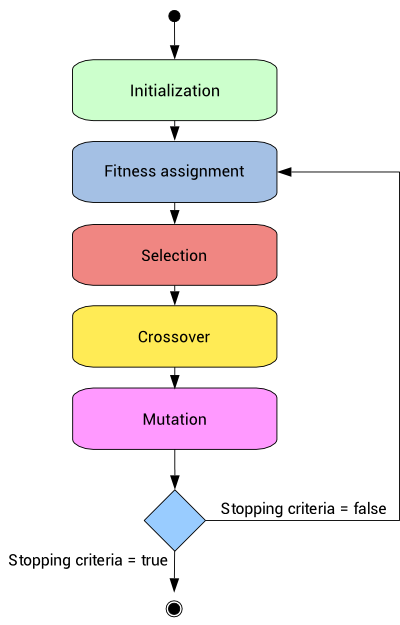
\includegraphics[width=0.6\linewidth]{3.png}
	\caption{\bf Process model for generating high diversity children based on input population.}
	\label{fig:GA_Model}
\end{figure}

Genetic Algorithm is heuristic optimization inspired by natural evolution. They can help in optimizing the performance of predictive model by selecting the most relevant features. The first step is to initialize the individuals in the population. As it is a stochastic optimization method, the genes of the individuals are initialized at random. Genes are nothing but the features of the population set. The next step is to assess the fitness of the individual. To evaluate fitness, a predictive model with training data needs to be trained and evaluate its selection error with the selection data. Selection error is nothing but the error of the model on an independent data set not used to create the model. Most used method for fitness assignment is rank based. The individuals are then ranked as per their selection error. The rank of the individual is multiplied with k also called selective pressure in order to obtain the fitness value. Individuals with low fitness values will be discarded.

After fitness selection, the individuals need to be chosen that will recombine for the next generation. Only a small group is chosen for recombination, and they are often selected randomly. The crossover function recombines to create new individuals until the population size is the same as the old population. Sometimes, crossover might generate children with the same features as that of the parents, which might cause low diversity. In order to avoid this, mutations are carried out on the offspring. They are done by randomly changing the feature of an offspring by flipping the feature of that individual.

\begin{figure}[H]
	\centering
	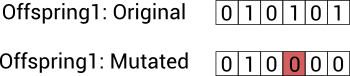
\includegraphics[width=0.4\linewidth]{4.png}
	\caption{\bf Mutating the features in an offspring to generate new population.}
	\label{fig:GA_Offspring}
\end{figure}

The rank of the individual is multiplied with k also called selective pressure in order to obtain the fitness value. Individuals with low fitness values will be discarded. After fitness selection, the individuals need to be chosen that will recombine for the next generation. Only a small group is chosen for recombination, and they are often selected randomly. The crossover function recombines to create new individuals until the population size is the same as the old population. Sometimes, crossover might generate children with the same features as that of the parents, which might cause low diversity. In order to avoid this, mutations are carried out on the offspring.

They are done by randomly changing the feature of an offspring by flipping the feature of that individual. Fitness evaluation, selection, crossover and mutation are done until certain criteria are met. The features will be assigned for the dataset obtained from NSE. The model will deliver high diversity children based on the input data.

By applying GA on given dataset, we can attempt to forecast the share prices.
GA has been applied using the Meyer-Packard algorithm. The Meyer and Packard algorithm is a genetic algorithm used for local forecasting of high dimensional chaotic systems and is based on functional optimization. In the example of a stock market prediction the algorithm would :

\begin{enumerate}
	\setstretch{1.5}
	\item Use past data as input as a set of {x, y} where x would be a multidimensional vector containing data like general market movement etc. and y a price representation
	\item Create an initial population of conditions C
	\item Evaluate each C based on past data (when C is true, what are the values for y) with a probability density function
	\item Apply crossover to the set of C\textquotesingle s. In this process two C elements with a high fitness value (i.e. evaluation) are picked and their data combined similar to the creation of new DNA from to strings of parent DNA
	\item Apply mutation. Randomly change certain C\textquotesingle s so that conditions not featured in the initial population can be created.
	\item Go to step 3 and repeat until model converges, i. e. C\textquotesingle s do not significantly change anymore.
\end{enumerate}

These refined Conditions C are then used to predict the market price at a given time. 

This method was applied in this project to forecast the CLOSE value by using values of NIFTY50 for 1 year worth data.

Firstly, the dataset is loaded onto the class called ``TrainingData''. Here all the column values of the .csv file are added to an individual list which holds value for each attribute. 

Then, the value for 1-day difference and the next day difference is calculated by subtracting OPEN and CLOSE for the respective days. Profit for holding a stock is also calculated by taking the difference for OPEN of current day and subtracting it from the OPEN of next day.

A population size of 200 is set. Using Normal distribution, the chromosomes are generated randomly and stored in an array as the randomly seeded population. After seeding the population, it must be subjected to fitness testing in order to ensure high accuracy of off springs. The values of chromosomes are compared to the 1-day and next day difference in order to estimate whether the selected specimen is useful or not. If the values of chromosomes of selected specimen are better than the actual values, it is selected as a profit estimation, else it is taken as a loss. If the chromosomes do not match the 1-day and next day criteria, it is assigned a default score.

After estimation of fitness, the new population is subjected to crossover. The population/parents for this part are selected randomly in order to ensure a more diverse output. During crossover, tow samples are selected randomly and subjected to crossover. Then the chromosomes of the samples are randomly generated again at a specified rate to induce mutation. Then the mutated samples are subjected to crossover again. Now an off spring is generated. This method gives yield to children which are varying in values from parents and are part of the new generation.

Finally, the values of the offspring are compared to original values of the 1-day and next day difference and stored in another .csv file as SCORE of the offspring. 

The values of SCORE and actual values are plotted to establish a comparison of the accuracy of the model. This is displayed in figure \ref{fig:GA_MPFinal}. 

\section{Random Forest}
Random Forest is a learning method for various tasks which works by constructing n decision trees at the time of training and giving an output which is the mean prediction of individual trees. 

It is better than other decision trees as it takes care of the problem of overfitting. Other than that, it has higher accuracy than other trees and even the cross-validation accuracy of a random forest is more than other decision tress. The random forest model will be created after collecting and pre-processing data. In this n-number of trees are constructed after training a data. These trees are created based on the various conditions of the subsets of data taken from the training set.


\begin{figure}[H]
	\centering
	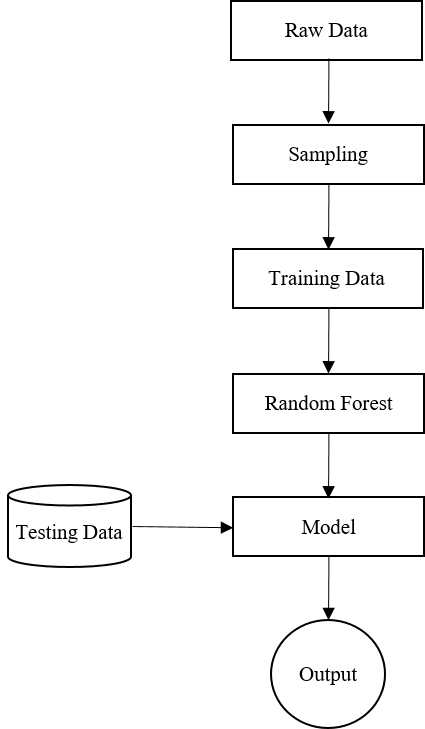
\includegraphics[width=0.4\linewidth]{Picture1.png}
	\caption{\bf Model for Random Forest Tree generation and output generate after model creation}
	\label{fig:RFModel}
\end{figure}

Random Forest can be used to create both short term and long term prediction models. The difference arises on which type of algorithm is used to train the model.
Random Forest Algorithm -

\begin{enumerate}
	\item Create n number of subset using Sample set.
	\item Decision Trees are created for each Subset using Information Gain and Entropy. 
	\item While selecting a node, votes are assigned to each attribute.
	\item Node with highest votes is selected as Key Node.
\end{enumerate}

It is a simple, flexible and easy to use algorithmic approach which provides consistent results most of the time, even without hyper-parameter tuning. It can be used for both classification and regression tasks. Most of the times it uses the bagging method to train the trees. The idea behind bagging is that a combination of learning models improves the overall result. 

It adds additional randomness to the model, while growing the trees. Instead of searching for the most important feature while splitting a node, it searches for the best feature among a random subset of features. This results in a wide diversity that generally results in a better model.

In this project a random forest model is implemented to predict the value of CLOSE. Using 1 year of values as training set, the model is created as given in figure (\ref{fig:RF_Attributes}).

At the start, all the necessary modules and functions are imported into the program.
Then, a plot of all attributes from the set is done in order to establish the relation between the label and the features that surround the label, and this is done using the module pyplot. Then all the attributes are compared to CLOSE to establish a relation. The attributes which can be used to predict the value of CLOSE are marked as features.



Then the data is split into training and testing. The split is taken as 80:20, where 80\% of the data is taken as training and the remaining 20\% is taken as testing set. 
A Random Forest model is then created. The model takes into account the 3 features and uses them to train itself to predict label CLOSE. A unit of 100 trees are created for the Forest model. This value of 100 can be increased to 200 or even reduced to 50.
But changing the number of tress has significant impact on how the model will be generated. Too many trees and the model will overfit and too few will cause the model to underfit.

After deploying the model, the 80\% of training data is fit into the model to predict CLOSE label. After fitting the model on training data, it is tested on the remaining 20\% data by predicting the model. 

Finally, a comparison is done between the predicted and actual values. The 2 values are plotted on a graph using the pyplot function. It is observed that the prediction values are quite close to the actual values. From figure \ref{fig:Output} it is clearly visible that the model displays high level of accuracy.

\section{Long Short Term Memory}

LSTM stands for Long Short Term Memory. It is a synthetic continual neural network, (RNN) design utilized in the sphere of deep learning. in contrast to normal RNNs, LSTM has feedback connections that build it a general purpose pc. It cannot solely method single information points (such as images), however additionally entire sequences of knowledge (such as speech or video). 

A common LSTM unit is composed of a cell, input, output and a forget gate. Data flows constantly throughout the cells and they keep track of relevant information and forget the unwanted information with each pass, which is handled by the 3 above mentioned gates. 

LSTM networks are well-suited to classifying, method and making predictions based on previous historic data, since there could also be lags of unknown length between very important events throughout a datum. LSTMs were developed to subsume the exploding and vanishing gradient problems which will be encountered once work ancient RNNs. Relative inability to gap length could be a bonus of LSTM over RNNs, hidden scientist models and different sequence learning ways in which in varied applications. 

Exemplary RNNs will monitor subjective long run conditions within the info arrangements. the problem of classic RNNs is procedure (or all the way down to earth) in nature: once making ready a vanilla RNN utilizing back-engendering, the angles that ar back-spread will disappear (that is, they\textquotesingle ll become normally zero) or detonate (that is, they\textquotesingle ll become infinity), as a results of the calculations related to the procedure, that utilize restricted accuracy numbers. RNNs utilizing LSTM units somewhat pay attention of the evaporating slope issue, on the grounds that LSTM units change inclinations to stay unchanged. Be that because it might, LSTM systems will in any case expertise the sick effects of the explosive angle issue even so. 

There unit of measurement several architectures of LSTM units. a typical style consists of a cell (the memory a district of the LSTM unit) and three ``regulators'', usually referred to as gates, of the flow of information inside the LSTM unit: degree input gate, degree output gate and a forget gate. Some variations of the LSTM unit haven\textquotedblleft t got one or tons of of these gates or maybe manufacture different gates. Intuitively, the cell is in command of keeping track of the dependencies between the weather inside the input sequence. The input gate controls the extent to it a replacement value flows into the cell, the forget gate controls the extent to it a worth remains inside the cell and conjointly the output gate controls the extent to it the value inside the cell is used to work the output activation of the LSTM unit. The activation operate of the LSTM gates is sometimes the logistic operate. 

There unit of measurement connections into and out of the LSTM gates, a number of that unit of measurement perennial. The weights of these connections, that need to be learned throughout work, verify but the gates operate. 

In this project, a LSTM model is enforced using Tensorflow and Keras APIs. TensorFlow is a software package library for dataflow and differentiable programming across a multitude of tasks. It\textquotesingle s a symbolic maths library, and is additionally used for machine learning applications like machine learning, statistical modelling, neural networks, deep learning etc. Keras on the other hand is used defining layers for neural network. It is simple and easy and implement. Keras can use Tensorflow functions and tends to work as a superclass over it.

Firstly, all required modules are imported into the program. This includes modules such as sklearn which help us in estimating performance metrics and keras which provides us with the LSTM layers. Then, the dataset is loaded into the program. 

In order to better train the module, the dataset scaled using a MinMaxScaler function. Since the values of the dataset range in 6-8 floating decimal values, it becomes difficult for the model to send the LSTM data across layers repeatedly. The scaler normalizes the values of dataset between 0 and 1. The first 60 entries in the dataset are used as features and from the 61st entry, it\textquotesingle s marked as label. The scaler is trained for values from the 61st entry.  

Then using Keras and Tensorflow, a sequential LSTM model is implemented. 
The model uses 1 layer of sequence, followed by 4 dropout layers and 1 dense layer. 
The model will be trained for 100 epochs and each epoch batch size is set as 32. The error estimation method is taken as MSE which is the Mean Squared Error. And optimizer which is used is ADAM.

The values of the batch and epoch size can be increased, however, the build time increases significantly.

The model takes time to build for 100 epochs. After the model is built, the training dataset is taken, which contains the values of the next year. In this case, the training dataset was taken from year 2016 and the testing data set is taken as 2017. 

Again, like with training set, the values are scaled so that they only range from 0 to 1. This is done to reduce the input of large floating point entries into the model which will only reduce the working speed of the model. After the data has been scaled, the model is fed the testing data. 

Finally, a plot of actual versus predicted values is done to display the accuracy of the model. This is shown in figure \ref{fig:LSTM_Output}

\pagebreak

\section{Auto Regressive Integrated Moving Average}

The ARIMA model is a time series based model which is a generalization of the ARMA model. Both ARMA and ARIMA can be used to better understand the data or to predict future points i.e. forecasting. 

The AR a part of ARIMA indicates that the evolving variable of interest is regressed on its own lagged (i.e., prior) values. The MA half indicates that the regression error is truly a linear combination of error terms whose values occurred contemporaneously and at numerous times within the past. The I (for ``integrated'') indicates that the information values are replaced with the distinction between their values and therefore the previous values (and this differencing method might are performed quite once). the aim of every of those options is to form the model match the information furthermore as attainable.

Non-seasonal ARIMA models area unit typically denoted denoted by variables p,q,d wherever parameters p, d, and q area integers, p is that the order of the autoregressive model, d is that the degree of, and q is that the order of the moving-average model. Seasonal ARIMA models area unit sometimes denoted using P, Q, D.

Also, purely autoregressive models resemble a linear regression output model.

ARIMA models work when only when the data set is stationary. A stationary data set means that the mean, variance and standard deviation from any selected point is the for all the values of the dataset. If a dataset is non stationary, then the ARIMA model will not work as the AR lags will be uneven. Also, ARIMA works best when the timestamp of the data is at regular intervals. The dataset might also turn out to be seasonal. Seasonal means that the there is a fixed pattern the values of the dataset which change depending on the season. Trend is another factor which is taken into consideration before building an ARIMA model. For only an ARIMA model, trend and seasonality must be eliminated, but for the Seasonal ARIMA mode; (SARIMA), only trend must be removed. 

But for both the models, the dataset in consideration must be stationary. In order to check whether the dataset is stationary or not there are certain methods. There are 2 used in this project and they are the ADF Test and Rolling Statistics. 
Rolling Statistics is a visual representation of the rolling mean and std. deviation with respect to the dataset used. It is a statistical calculation of the mean and std. deviation of the original dataset and is represented using plots on graph. For any given dataset on which rolling statistics are applied, the more linear the line for mean and std. deviation, the better the result. A linear or near linear line indiacates that the dataset is stationary. But a visual representation might not be exactly accurate. In order to get a definite result, the ADF test is used. ADF test stands for Augmented Dickey Fueller Test. The ADF test is used to evaluate whether the data is stationary or not. ADF is statistical evaluation that tests the null hypothesis that a unit root is present in a time series sample. When performed on any dataset it returns the ADF statistic value and the p value. The p value is used to test whether the hypothesis holds true or not.


\begin{itemize}
	\item The null hypothesis states that if the value of p<0.05, then the data is stationary. 
	\item The alternate hypothesis states that if p>0.05, then data is non-stationary.
\end{itemize}

Making the data stationary is very important else the model will not be generated.

After checking the model for stationarity, the trends and seasonality must be eliminated from the data. Trends and seasonality can become part of a dataset because of the recurring values at certain points. Since the data exists over a specific time period (days/months/years/decades etc.), there may be chance that values repeat over seasons. Trend refers to an upward increase in the values of the dataset. Trend may be dampened, exponential etc. To ensure an ARIMA model gives accurate results, trend and seasonality must be eliminated from the dataset. In order to eliminate trend and season, there are various methods but they depend on the type of trend or seasonality. 

When eliminating trends and seasonality, the dataset might be subjected to various levels of differencing such as 1-day differencing etc. If the initial dataset isn\textquotesingle t stationary, the dataset is transformed into a stationary one by means of differencing. The amount of times differenced is the value which is taken as `d' in the ARIMA model. Based on the trend the dataset is subjected to log differencing or root differencing. 

After the dataset is confirmed to be stationary and trends and seasonality are eliminated, the next step is to estimate the AR and MA values of which will be input into the model. The AR and MA values are found out using the ACF and PACF plots which are the representation of the lags. The first lag which touches the upper confidence interval is taken the AR and MA value. The value could be any integer and it purely depends on the dataset used and the amount of differencing done on it.

In this project, the values form year 2016 are taken as the base from which the values of next 15 units will be forecasted. 

As explained above the dataset is tested for stationarity using the rolling statistics and ADF test right away as shown in figure \ref{fig:ARIMA_Original}.

From the graph it is clearly visible that the dataset is not stationary and that there is dampened trend on it. The ACF of the data is taken to check whether we could determine the AR value.

From the ACF plot in figure \ref{fig:ARIMA_ACFOri}, it is visible that the dataset is not stationary as the lags move far into the negative zone. The moving average of the dataset is also plotted as shown in figure \ref{fig:ARIMA_MAFOri}

Then, mean of the first 12 values is subtracted from the rest of the data. The log transform of the data is also taken. Then the log transform of the data is subtracted from the mean taken previously. This is the moving average of the original set.

A log transform is performed to eliminate the trend. Then rolling stats and ADF test is performed again on the log transformed values and the p value is checked again. The value of p>0.05, which indicates that the dataset is non stationary in nature.

The plot of Rolling Statistics vs Log Transform is given as in figure \ref{fig:ARIMA_ARIMA_RSLog}.

Another approach is then taken. This time a log shift is taken instead of the log differencing. A log shift means subtracting the next value from the previous. Then the ADF test and Rolling Statistics are performed again as done in figure \ref{fig:ARIMA_RSLogDiff}).

However, now we see that value of p has reduced to 0 but our dataset looks more linear than before and that the mean and std. deviation are almost linear. 

Then the ACF and PACF values are plotted in figure \ref{fig:ARIMA_ACFLogDiff} and figure \ref{fig:ARIMA_PACFLogDiff} to estimate the AR and MA for this data.

Based on the plots, the AR and MA values are taken as 1,1 and the differencing is also taken as 1. Also, by using ndiffs, the best value for differencing is calculated, which is returned as 1.

Hence, an ARIMA model of (1,1,1) is taken for forecasting. A plot of the forecasted vs actual values is done. This is obtained in figure \ref{fig:ARIMA_Final}

The model is clearly unable to work on this dataset and hence the values are closer to 0 and some even negative. This is due to the fact that the log shift is not a feasible method to eliminate trend for this dataset. \pagebreak

\chapter{SCREENSHOTS}

\begin{figure}[H]
	\centering
	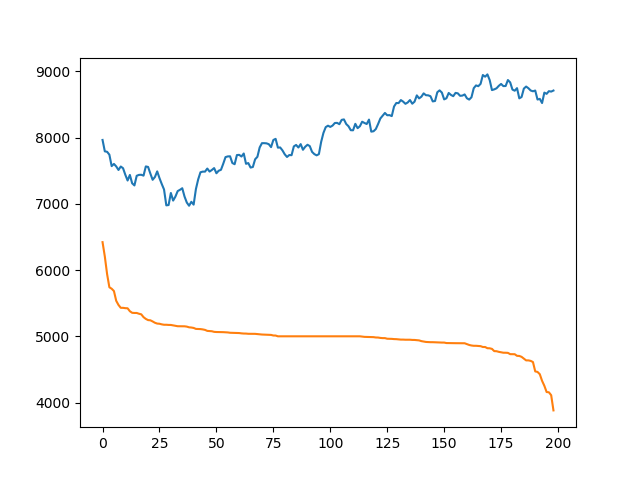
\includegraphics[width=\linewidth]{GA_MPFinal.png}
	\caption{\bf Plot of CLOSE values estimated by GA model and the actual CLOSE values.}
	\label{fig:GA_MPFinal}
\end{figure}

\begin{figure}[H]
	\flushleft
	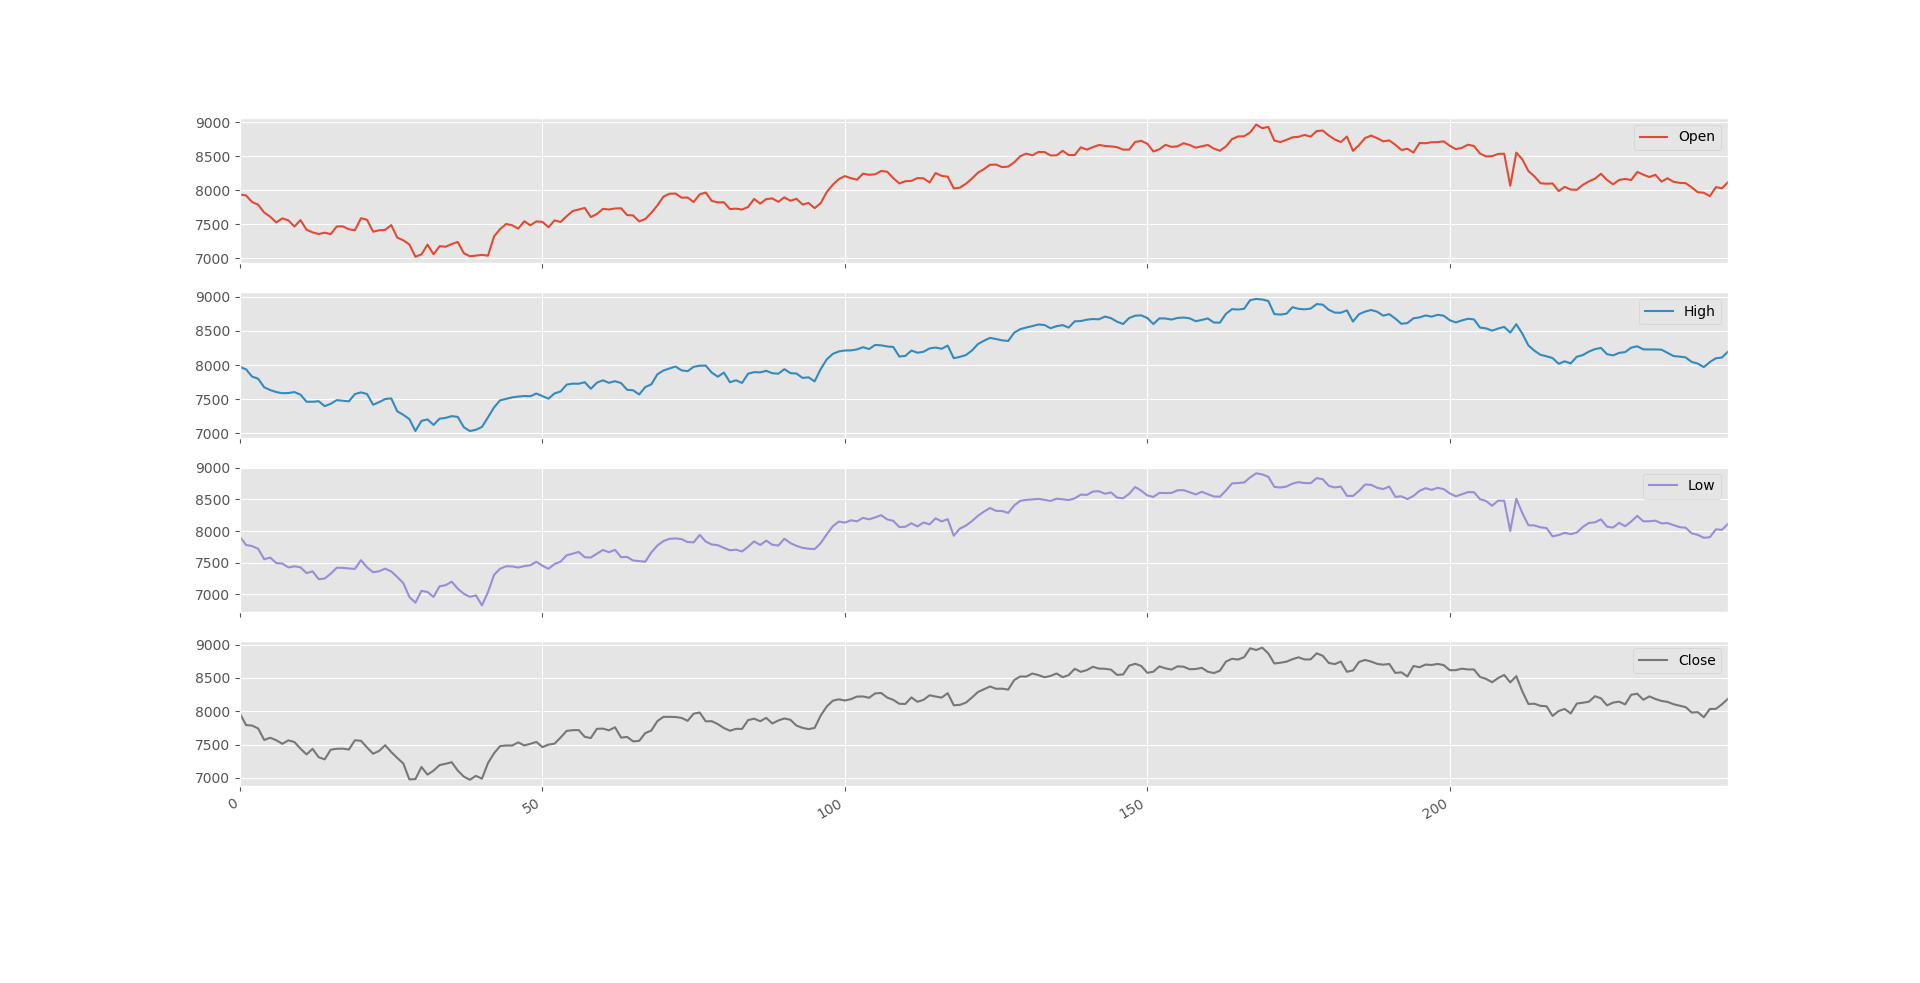
\includegraphics[width=\linewidth]{RF_Attributes.png}
	\caption{\bf Plot of all attributes}
	\label{fig:RF_Attributes}
\end{figure}

\begin{figure}[H]
	\centering
	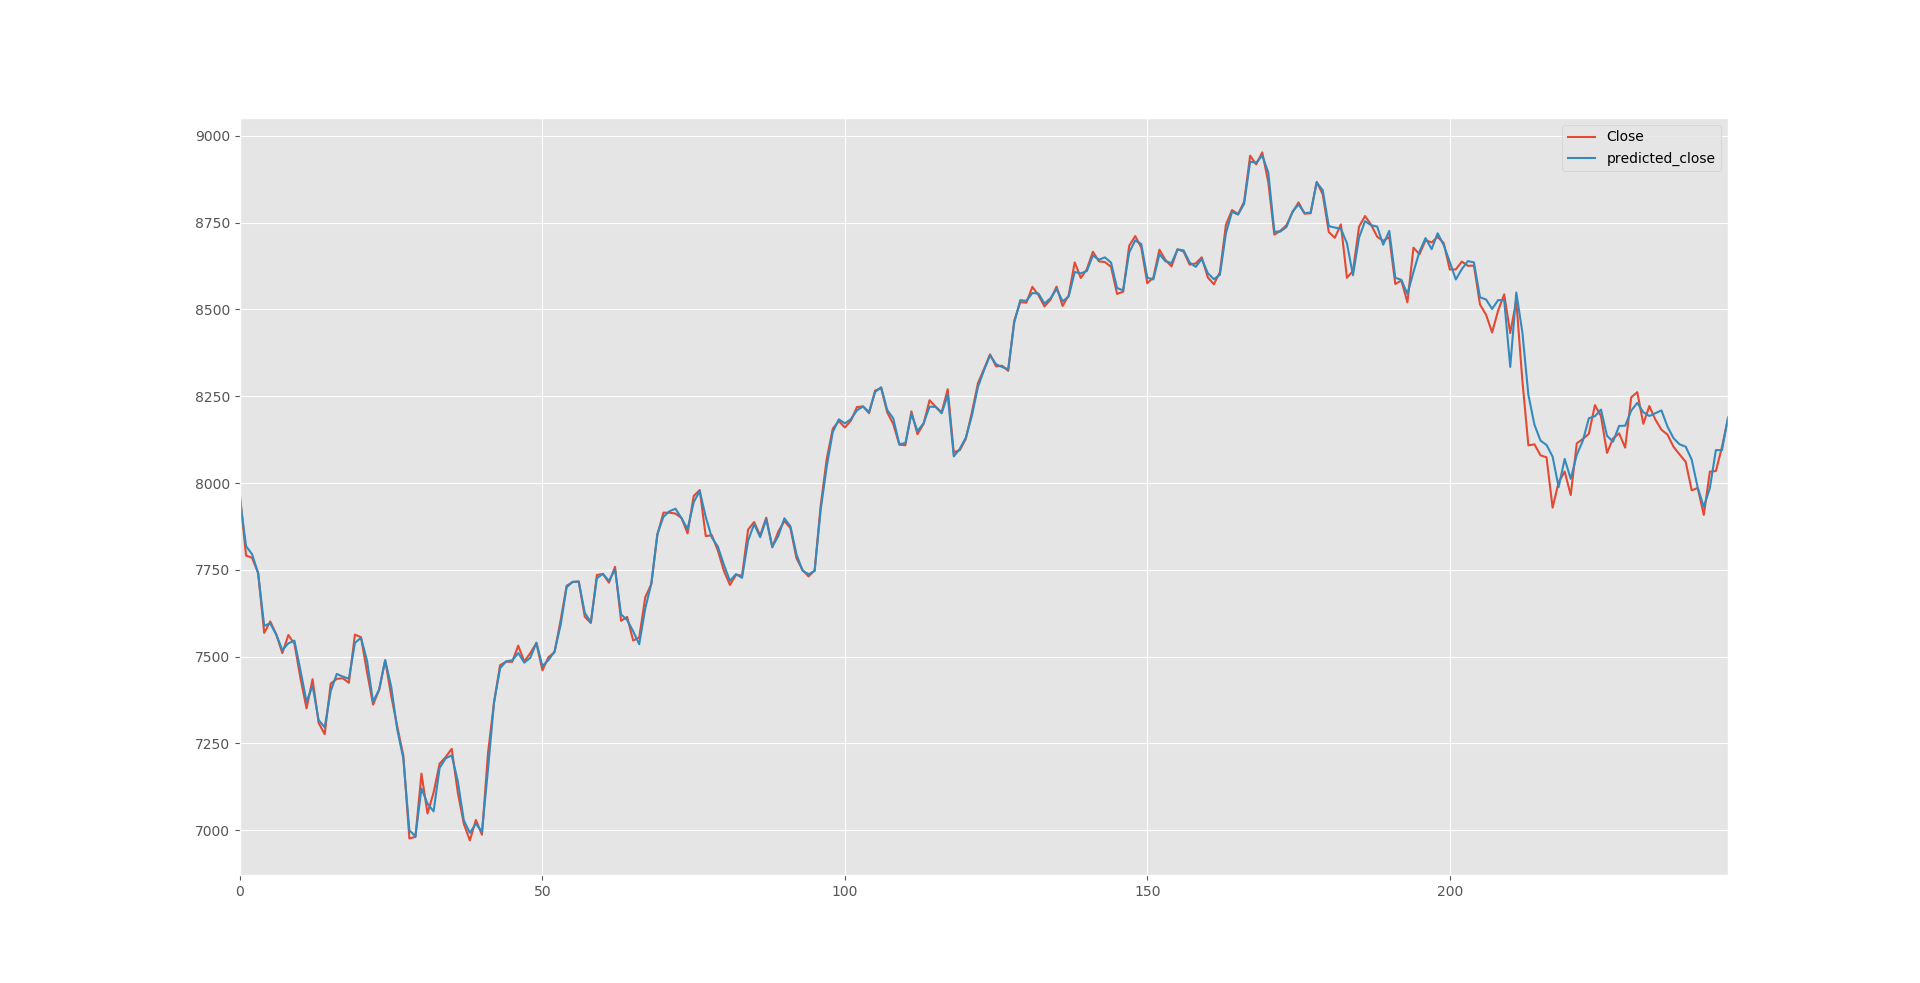
\includegraphics[width=\linewidth]{RF_OutputPlot.png}
	\caption{\bf Plot of predicted prices vs actual values for Random Forest Model}
	\label{fig:Output}
\end{figure}

\begin{figure}[H]
	\centering
	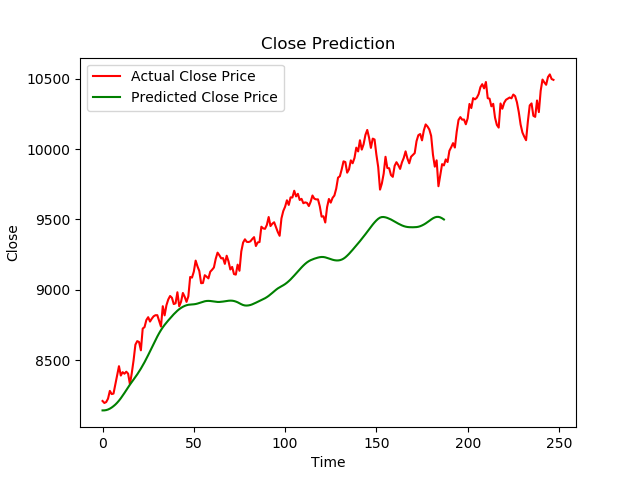
\includegraphics[width=\linewidth]{LSTM_Final.png}
	\caption{\bf Plot of predicted prices vs actual values for LSTM Model}
	\label{fig:LSTM_Output}
\end{figure} 

\begin{figure}[H]
	\centering
	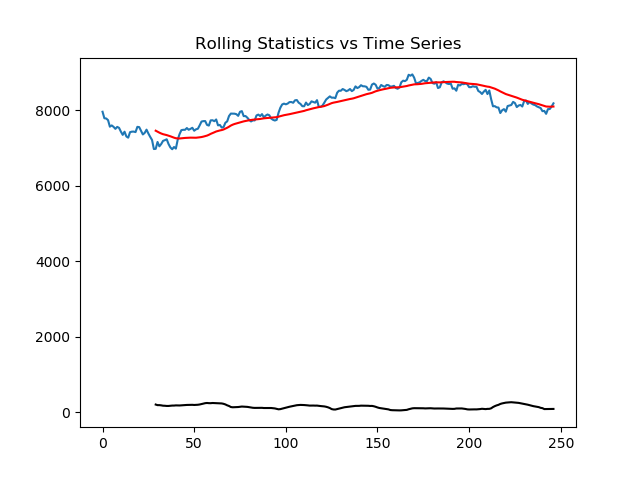
\includegraphics[width=\linewidth]{ARIMA_RSOri.png}
	\caption{\bf Rolling Statistics for original dataset}
	\label{fig:ARIMA_Original}
\end{figure} 

\begin{figure}[H]
	\centering
	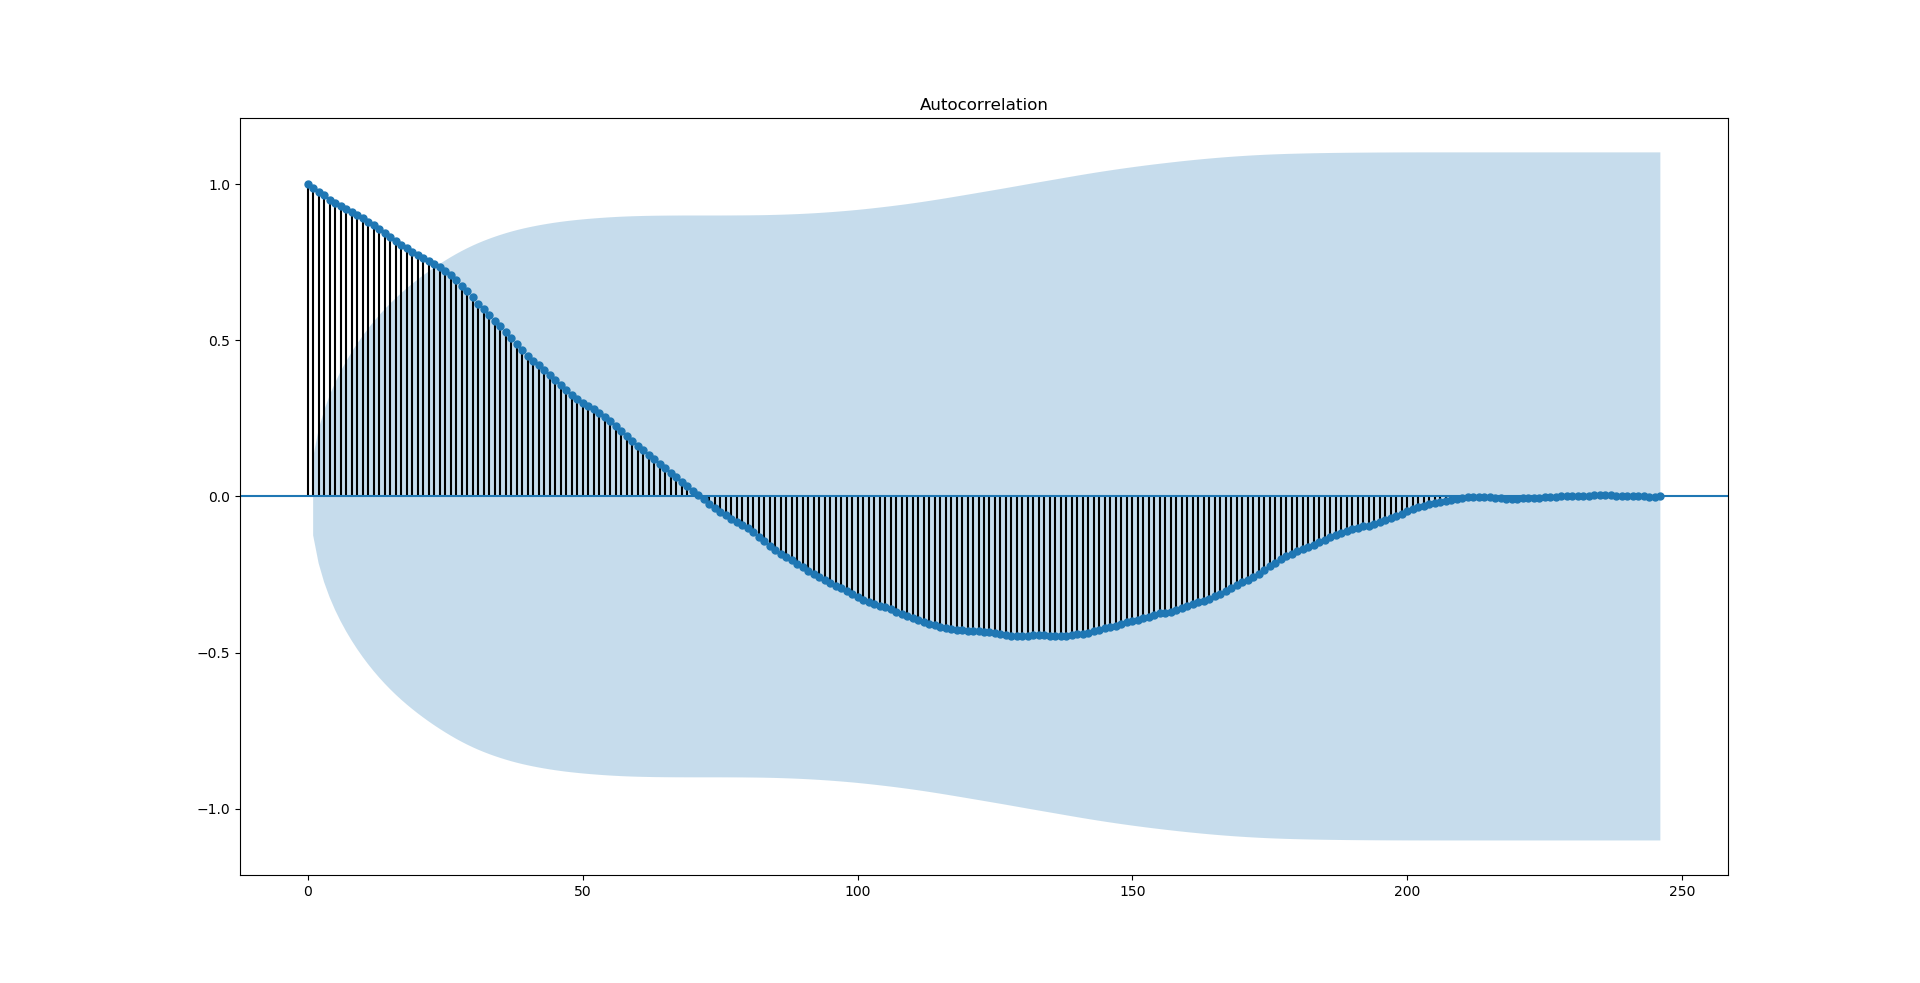
\includegraphics[width=\linewidth]{ARIMA_ACFOri.png}
	\caption{\bf ACF for the original dataset}
	\label{fig:ARIMA_ACFOri}
\end{figure}

\begin{figure}[H]
	\centering
	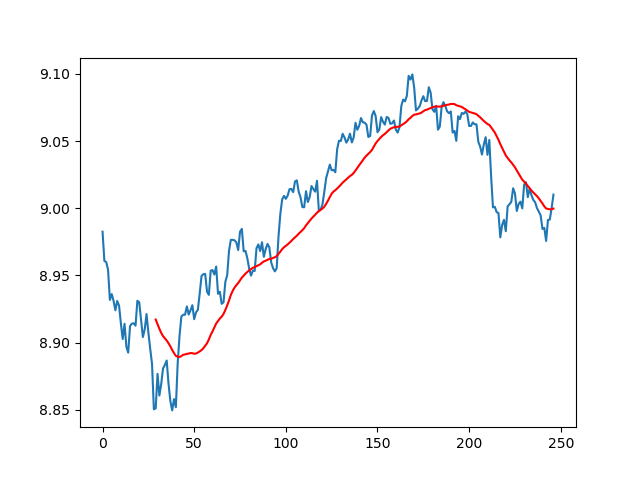
\includegraphics[width=\linewidth]{ARIMA_MAOri.png}
	\caption{\bf Moving Average of the original dataset}
	\label{fig:ARIMA_MAFOri}
\end{figure}

\begin{figure}[H]
	\centering
	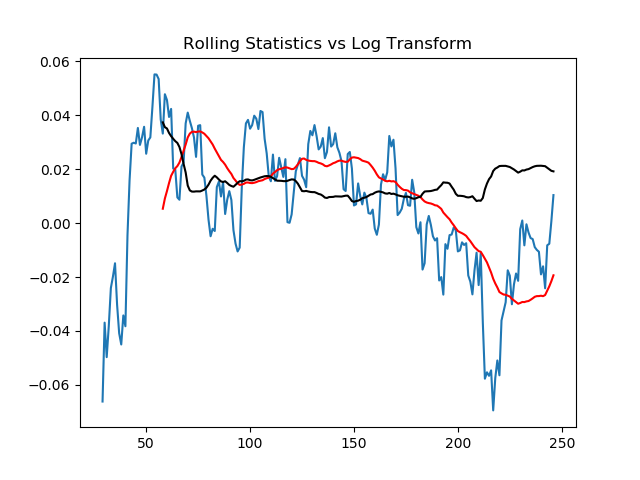
\includegraphics[width=\linewidth]{ARIMA_RSLog.png}
	\caption{\bf Rolling Statistics vs Log Transform}
	\label{fig:ARIMA_ARIMA_RSLog}
\end{figure}

\begin{figure}[H]
	\centering
	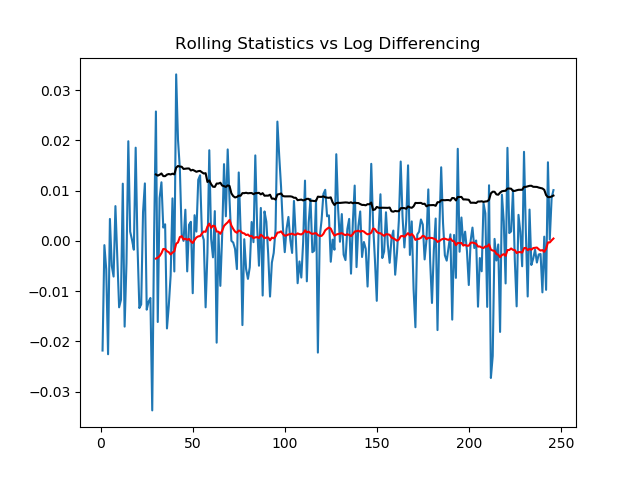
\includegraphics[width=\linewidth]{ARIMA_RSLogDiff.png}
	\caption{\bf Rolling Statistics vs Log Differencing}
	\label{fig:ARIMA_RSLogDiff}
\end{figure}

\begin{figure}[H]
	\centering
	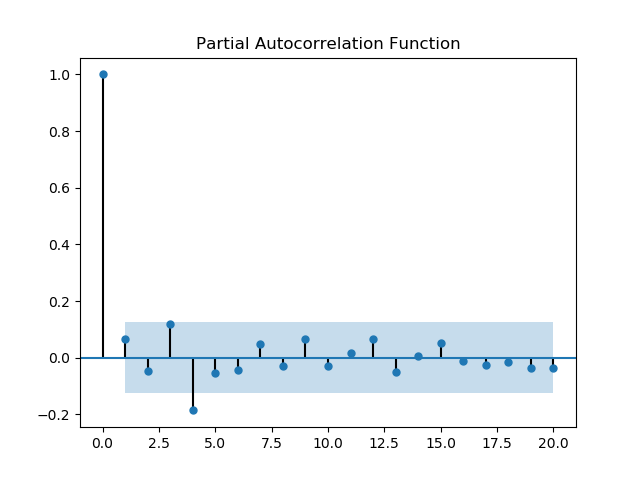
\includegraphics[width=\linewidth]{ARIMA_ACFLogDiff.png}
	\caption{\bf ACF Plot of the Log Differenced}
	\label{fig:ARIMA_ACFLogDiff}
\end{figure}

\begin{figure}[H]
	\centering
	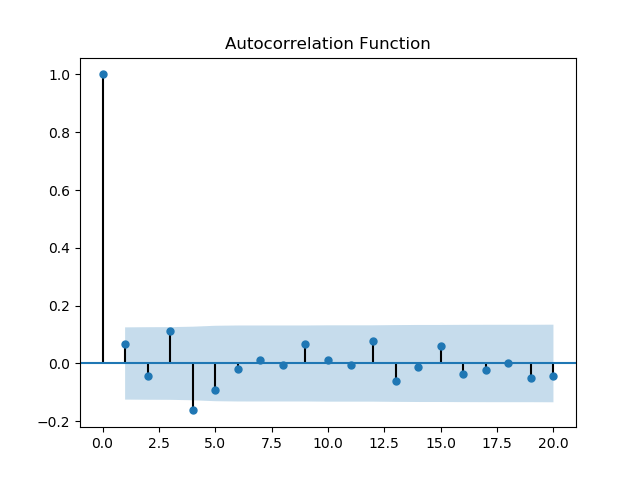
\includegraphics[width=\linewidth]{ARIMA_ACFLogDiff1.png}
	\caption{\bf PACF Plot of Log Differenced}
	\label{fig:ARIMA_PACFLogDiff}
\end{figure}

\begin{figure}[H]
	\centering
	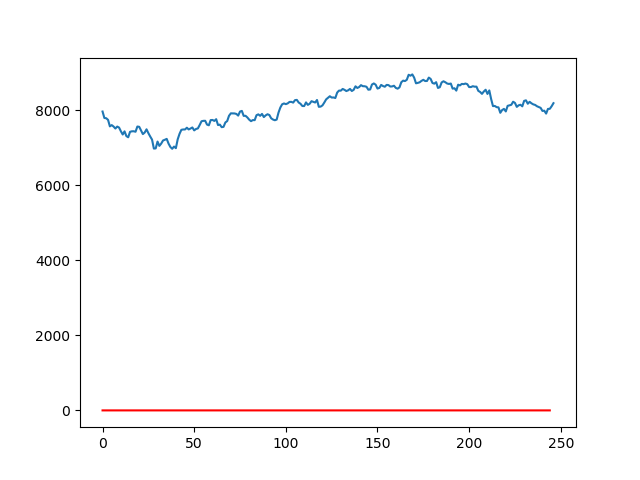
\includegraphics[width=\linewidth]{ARIMA_Final.png}
	\caption{\bf Final Plot of ARIMA forecasted values vs actual values}
	\label{fig:ARIMA_Final}
\end{figure}


\chapter{CONCLUSION}

The project was undertaken in an attempt to improve the prediction accuracy of the various exitsting models. Throughout the duration of the project various models were which used different apporaches with respect to prediction of future values.

The objective of the project was to work on existing models and compare their accuracy values. This was attempted by using the same dataset across all models.
All dataset values were taken from \ac{NIFTY50}. 

All models were implemented sucessfuly with the exception of ARIMA model which produced poor results due to unsucessful processing of dataset. 

Mean Square Error (MSE) is the metric that is used and deployed across all models in order to have a uniform performance estimation parameter. MSE is calculated by subtracting the original from the predicted values and taking the mean of their squares.

The MSE for all models has been displayed in the table given below.

\begin{table}[H]
	\centering
	\begin{tabular}{|c|c|c|}
		\hline
		\bf Model Used & \bf MSE \\
		\hline
		Genetic Algorithm & 9748087.5567\\	
		\hline
		Random Forest & 736.9183\\	
		\hline
		LSTM & 1153155.5518\\	
		\hline
		ARIMA & NA\\	
		\hline
	\end{tabular}
	\caption{\bf Table displaying the MSE values for all the models implemented.}
\end{table}

From the above data, it is clearly visible that Random Forest model has the least MSE in comparison to the others.

But, it can be noted from the graphs of the other models that their forecasts were unstable and non uniform. Hence, an argument can be made that their error estimation is more than it should be. For instance in figure \ref{fig:LSTM_Output}, it can be clearly observed that the forecasted values move far away from the actual values. This leads to a greater error difference and hence the MSE value increases. The same observation could be made for figure \ref{fig:GA_MPFinal}.


\chapter{FUTURE ENCHANCEMENTS}

The accuracy of the models can certainly be improved in order to obtain better results. By changing parameters or by additional training methods and constraints, they can be further.

Random Forest alraedy provides us with an accurate result.
For the various models trained and tested, Random Forest displayed the best prediction accuracy. The models of Genetic Algorithm, Long Short Term Memory and ARIMA produced poor results than Forest. Though LSTM fared significantly better than GA based model or ARIMA which displayed negligible result.
The models can be improved as -

\begin{enumerate}
	\setstretch{1.5}	
	\item Auto Regressive Integrated Moving Average (ARIMA)
	\begin{itemize}
	\setstretch{1.5}
		\item Performing more data processing to eliminate trend, seasonality and non-stationarity
		\item Also selecting data such that the frequency of time units is constant over time
	\end{itemize}
	\item Long Short Term Memory (LSTM)
	\begin{itemize}
		\setstretch{1.5}
		\item Using more layers to further improving accuracy
		\item Increasing the batch size
		\item Using correct weights after analysing instead of a random seed
		\item The model accuracy is also limited by performance of the harware in use. In this instance, the model was trained at 100 epochs, which if increased may certainly yield a better model as the model will be trained more on the dataset.
	\end{itemize}
	\item Genetic Algorithm (GA)
	\begin{itemize}
		\setstretch{1.5}
		\item Using Machine Learning models to further improve the offspring generation
		\item By applying a GA based apporoach on any other model could also be implmented. For instance, by using a fitness function to evaluate the best weights in a neural network based model
	\end{itemize}
\end{enumerate}

\appendix
\chapter{CODE}
\section{Genetic Algorithm}

\lstset{%
	breaklines=true,
	breakatwhitespace=true,
}
\begin{lstlisting}
#Import required modules
import numpy
import random
import operator
import csv
import pandas
import matplotlib.pyplot as plt
from sklearn.metrics import mean_absolute_error, mean_squared_error


# Set constants
random.seed(a=None)
PopulationSize = 200
DataSize = 0
MutationRate = 0
NumReturn = 5
File_path = 'closePrices.csv'


class Chromosome():
def __init__(self, min=None, max=None, prev_min=None, prev_max=None, buy=None, score =None):
self.min = min
self.max = max
self.prev_min = prev_min
self.prev_max = prev_max
self.buy = buy
self.score = score

DataSize = len(self.dayChange)

#Initializes the population of random chromosomes
def populationInit(self):

#Create N Chromosomes with N being the Population Size
#Each variable of Chromosome is assigned a number from a normal distribution
#with the mean being 0 and the Standard Deviation being 0.15

mu, sigma = 0, 0.15 # mean and standard deviation
s = numpy.random.normal(mu, sigma, 4*PopulationSize)
x = iter(s)
for i in range(PopulationSize):
temp = Chromosome(next(x),next(x),next(x),next(x),random.randint(0,999)%2, 0)

#If the mininum is assigned a higher value than the max swap them
#so that it makes sense.
if temp.min > temp.max:
temp.min, temp.max = temp.max, temp.min
if temp.prev_min > temp.prev_max:
temp.prev_min, temp.prev_max = temp.prev_max, temp.prev_min

#Push the Chromosome into the population array.
self.population.append(temp)

#Determines score for each chromosome in self.population
def fitnessFunction(self):
for i in range(len(self.population)):
match = False
for j in range(DataSize):

#BUY
if(self.population[i].prev_min < self.dayChange[j] and self.population[i].prev_max > self.dayChange[j]):
if(self.population[i].min < self.nextDayChange[j] and self.population[i].max > self.nextDayChange[j]):
if(self.population[i].buy == 1):
match = True
self.population[i].score += self.profit[j]

#SELL
if(self.population[i].prev_min < self.dayChange[j] and self.population[i].prev_max > self.dayChange[j]):
if(self.population[i].min < self.nextDayChange[j] and self.population[i].max > self.nextDayChange[j]):
if(self.population[i].buy == 0):
match = True
self.population[i].score -= self.profit[j]

if match == False:
self.population[i].score = -5000

#Weighted random choice selection
def weighted_random_choice(self):
self.fitnessFunction()
max = self.population[0].score
for i in self.population[1:]:
max+= i.score
pick = random.uniform(0,max)
current = 0
for i in range(len(self.population)):
current += self.population[i].score
if current > pick:
self.nextGeneration.append(self.population[i])

#Removes the indices in self.population that have a score of None
def exists(self):
i = 0
while i <len(self.population):
if self.population[i].score is None:
del self.population[i]
else:
i+=1

#Uniform Crossover
def uniformCross(self, z):
children = []
for i in range(PopulationSize-len(self.nextGeneration)):
child = Chromosome(0,0,0,0,0)
chromosome1 = self.nextGeneration[random.randint(0,999999) % len(self.nextGeneration)]
chromosome2 = self.nextGeneration[random.randint(0,999999) % len(self.nextGeneration)]
if(random.randint(0,999) %2):
child.min = chromosome1.min
else:
child.min = chromosome2.min

if(random.randint(0,999) %2):
child.max = chromosome1.max

else:
child.max = chromosome2.max

#Append
children.append(child)

def csv_dict_writer(self,path, fieldnames, data):
out_file  = open(path, "wb")
df = pandas.DataFrame(data)
df.to_csv(path)


if __name__ == '__main__':
x = TrainingData()
x.generateData()
x.populationInit()
x.weighted_random_choice()
x.uniformCross(MutationRate)
x.printChromosomes()

data = pandas.read_csv('2016.csv', nrows=199)
data = data[['Close']]

data_predicted = pandas.read_csv('closePrices.csv')
data_predicted = data_predicted[['Score']]
plt.plot(data)
plt.plot(data_predicted)
plt.show()

mape = mean_absolute_error(data, data_predicted)
mse = mean_squared_error(data, data_predicted)

# Print MAE, MAPE and Accuracy
print('Mean Squared Error - ', mse)
print('Mean Average Percent Error - ', mape)
\end{lstlisting}
\pagebreak

\section{Random Forest}

\lstset{%
	breaklines=true,
	breakatwhitespace=true,
}
\begin{lstlisting}
#Import required modules
import numpy as np
from math import sqrt
import pandas as pd
import matplotlib.pyplot as plt
from sklearn.ensemble.forest import RandomForestRegressor
from sklearn.metrics import mean_absolute_error, mean_squared_error

#Open dataset to read from
data = pd.read_csv('2016.csv')
data = data[['Open','High','Low','Close']]

#Plot all the concerned attributes to establish correlation
plt.rcParams['figure.figsize']=(20,10)
plt.style.use('ggplot')
data.plot(subplots=True)
plt.show()

#Split dataset attributes into features and prediction label
dX = data[['Open','High','Low']]
dy = data[['Close']]

#Split data into train and test
dX_train = dX[dX.index < 181]
dy_train = dy[dy.index < 181]

dX_test = dX[dX.index >= 181]
dy_test = dy[dy.index >= 181]

#Initiate Random Forest Model which makes use of 3 features to predict 'Close' for given data
RF_Model = RandomForestRegressor(n_estimators=100, max_features=3, oob_score=True)

#Fit data into the model
#Set 'Close' as the label to predict
label = dy_train[:]
features = dX_train[:]
rgr=RF_Model.fit(features, label)

#Using training features, predict the 'Close' value and store data into file
dX_test_predict=pd.DataFrame(
rgr.predict(dX_test[:])).rename(
columns={0:'predicted_close'}).set_index('predicted_close')
dX_train_predict=pd.DataFrame(
rgr.predict(dX_train[:])).rename(
columns={0:'predicted_close'}).set_index('predicted_close')

#Add predict values to the forest and append
RF_predict = dX_train_predict.append(dX_test_predict)

#Display file with new column of 'predicted_close'
data = data.join((RF_predict.reset_index()))
print(data.head())

#Plot 'Close' vs 'predicted_close'
data[['Close','predicted_close']].plot()
plt.show()

#Calculate the Mean Squared Error
data['Diff']=data.predicted_close - data.Close
data['Diff'].plot(kind='bar')
plt.show()

#Calculate the Mean Absolute Percent Error
dy_true = data[['Close']]
dy_predicted = data[['predicted_close']]
mape = mean_absolute_error(dy_true,dy_predicted)
mse = mean_squared_error(dy_true,dy_predicted)

#Print MAE, MAPE and Accuracy
print('Mean Squared Error - ',mse)
print('Mean Average Percent Error - ',mape)
\end{lstlisting}
\pagebreak

\section{Long Short Term Memory}

\lstset{%
	breaklines=true,
	breakatwhitespace=true,
}

\begin{lstlisting}
#Import required modules
import numpy as np
import matplotlib.pyplot as plt
import pandas as pd
from sklearn.preprocessing import MinMaxScaler
from sklearn.metrics import mean_absolute_error, mean_squared_error
from keras.models import Sequential
from keras.layers import Dense
from keras.layers import LSTM
from keras.layers import Dropout

#Load the required dataset
dataset_train = pd.read_csv('2016.csv')
training_set = dataset_train.iloc[:, 4:5].values
print(dataset_train.head())

#Scaling the data using MinMax scaler
MMScl = MinMaxScaler(feature_range = (0, 1))
training_set_scaled = MMScl.fit_transform(training_set)

#Using the first 60 stamps as features
#Using the 61 stamp onwards as label
X_train = []
y_train = []
for i in range(60, 247):
X_train.append(training_set_scaled[i-60:i, 0])
y_train.append(training_set_scaled[i, 0])
X_train, y_train = np.array(X_train), np.array(y_train)

X_train = np.reshape(X_train, (X_train.shape[0], X_train.shape[1], 1))

#Load the testing data set.
dataset_test = pd.read_csv('2017.csv')
real_stock_price = dataset_test.iloc[:, 1:2].values

#Concatenate the testing set to match the values for training set
#Then scale, reshape and fit the data into model
dataset_total = pd.concat((dataset_train['Close'], dataset_test['Close']), axis = 0)
inputs = dataset_total[len(dataset_total) - len(dataset_test) - 60:].values
inputs = inputs.reshape(-1,1)
inputs = MMScl.transform(inputs)
X_test = []
for i in range(60, 248):
X_test.append(inputs[i-60:i, 0])
X_test = np.array(X_test)
X_test = np.reshape(X_test, (X_test.shape[0], X_test.shape[1], 1))

#Create a prediction model based on testing data
predicted_stock_price = regressor.predict(X_test)
predicted_stock_price = MMScl.inverse_transform(predicted_stock_price)

#Estimate the MSE and MAPE between the real and predicted values
data = pd.read_csv('2016.csv', nrows=188)
dy_true = data[['Close']]
dy_predicted = predicted_stock_price
mape = mean_absolute_error(dy_true,dy_predicted)
mse = mean_squared_error(dy_true,dy_predicted)

#Print MAE, MAPE and Accuracy
print(mse)
print(mape)
\end{lstlisting}
\pagebreak

\section{Auto Regressive Intergrated Moving Average}

\begin{lstlisting}
#Import required modules
import math
import numpy as np
import pandas as pd
import matplotlib.pyplot as plt
import sklearn
import statsmodels.tsa.seasonal as sm
from statsmodels.tsa.stattools import adfuller
from statsmodels.graphics.tsaplots import plot_acf, plot_pacf
from statsmodels.tsa.seasonal import seasonal_decompose
from statsmodels.tsa.arima_model import ARIMA
from statsmodels.tsa.statespace import sarimax
from sklearn.metrics import mean_absolute_error, mean_squared_error
from pmdarima.arima.utils import ndiffs

#Load dataset and plot
data = pd.read_csv('2016.csv')
data = data[['Open','High','Low','Close']]

#Plot the label we want to predict and check for its seasonality
#Seasonality can be predicted using statistical methods or ADF test
#In this module, the ADF test has been taken, as it is more accurate in assessing whether the data is stationary or not.
rolmean = data.Close.rolling(30).mean()
rolstd = data.Close.rolling(30).std()
plt.plot(data.Close)
plt.plot(rolmean,color='red')
plt.plot(rolstd, color='black')
plt.title('Rolling Statistics vs Time Series')
plt.show()
result = adfuller(data.Close, autolag='AIC')
print('ADF Statistic: %f'% result[0])
print('p-value: %f'% result[1])
print('#Lags Used: ', result[2])
print('Observations Used: ', result[3])
print('Critical Values:')
for key, value in result[4].items():
print('\t%s: %.3f' % (key, value))

#Plot the ACF value
plot_acf(data.Close)
plt.show()

#Prints the required order of differencing to make the data stationary
#The suggested value may not be the best differencing for the dataset
#However, using more than the suggested difference will make the data overstationary and unfit for use
print('Best value of difference to use is - ',ndiffs(data.Close,test='adf'))

#Plot MA of the log
data1 = np.log(data[['Close']])
moving_avg = data1.rolling(30).mean()
plt.plot(data1)
plt.plot(moving_avg, color='red')
plt.show()

#Take the moving average of the data by subtracting the moving average for 30 time units from the original data
series_ma = data1 - moving_avg
series_ma.dropna(inplace=True)

#Perform order differencing based on ndiffs using .shift() method
ts_log_diff = data1 - data1.shift()
ts_log_diff.dropna(inplace=True)
plt.plot(ts_log_diff)
plt.title('After Log Differencing')
plt.show()
rolmean = ts_log_diff.rolling(30).mean()
rolstd = ts_log_diff.rolling(30).std()
plt.plot(ts_log_diff)
plt.plot(rolmean,color='red')
plt.plot(rolstd, color='black')
plt.title('Rolling Statistics vs Log Differencing')
plt.show()
ts_log_diff = ts_log_diff.iloc[:,0].values
result = adfuller(ts_log_diff, autolag='AIC')
print('ADF Statistic: %f' % result[0])
print('p-value: %f'% result[1])
print('#Lags Used: ', result[2])
print('Observations Used: ', result[3])
print('Critical Values:')
for key, value in result[4].items():
print('\t%s: %.3f' % (key, value))

#Plot ACF:
plot_acf(ts_log_diff, lags=20)
plt.title('Autocorrelation Function')

#Plot PACF:
plot_pacf(ts_log_diff, lags=20, method='ols')
plt.title('Partial Autocorrelation Function')
plt.show()

#Print MAE, MAPE and Accuracy
print('Mean Squared Error - ',mse)
print('Mean Average Percent Error - ',mape)
print('Estimated Accuracy - ',(100-mape))
\end{lstlisting}
\pagebreak
%%%%%%%%%%%%%%%%%%%%%%%%%%%%%%%%%%%%%%%%%%%%%%%%%%%%%%%%%%%%
% Bibliography.
\bibliographystyle{unsrtnat}
\bibliography{references}
%%%%%%%%%%%%%%%%%%%%%%%%%%%%%%%%%%%%%%%%%%%%%%%%%%%%%%%%%%%%
\end{document}